\section{Treating color images}

In exercise 6, the pixels showing a hand are extracted from the black background of an image and copied onto a second image. The commands used for this process can be found in \texttt{exercise6.m}. The resulting image is depicted in figure \ref{fig:task22}.

\begin{figure}[!hbt]
  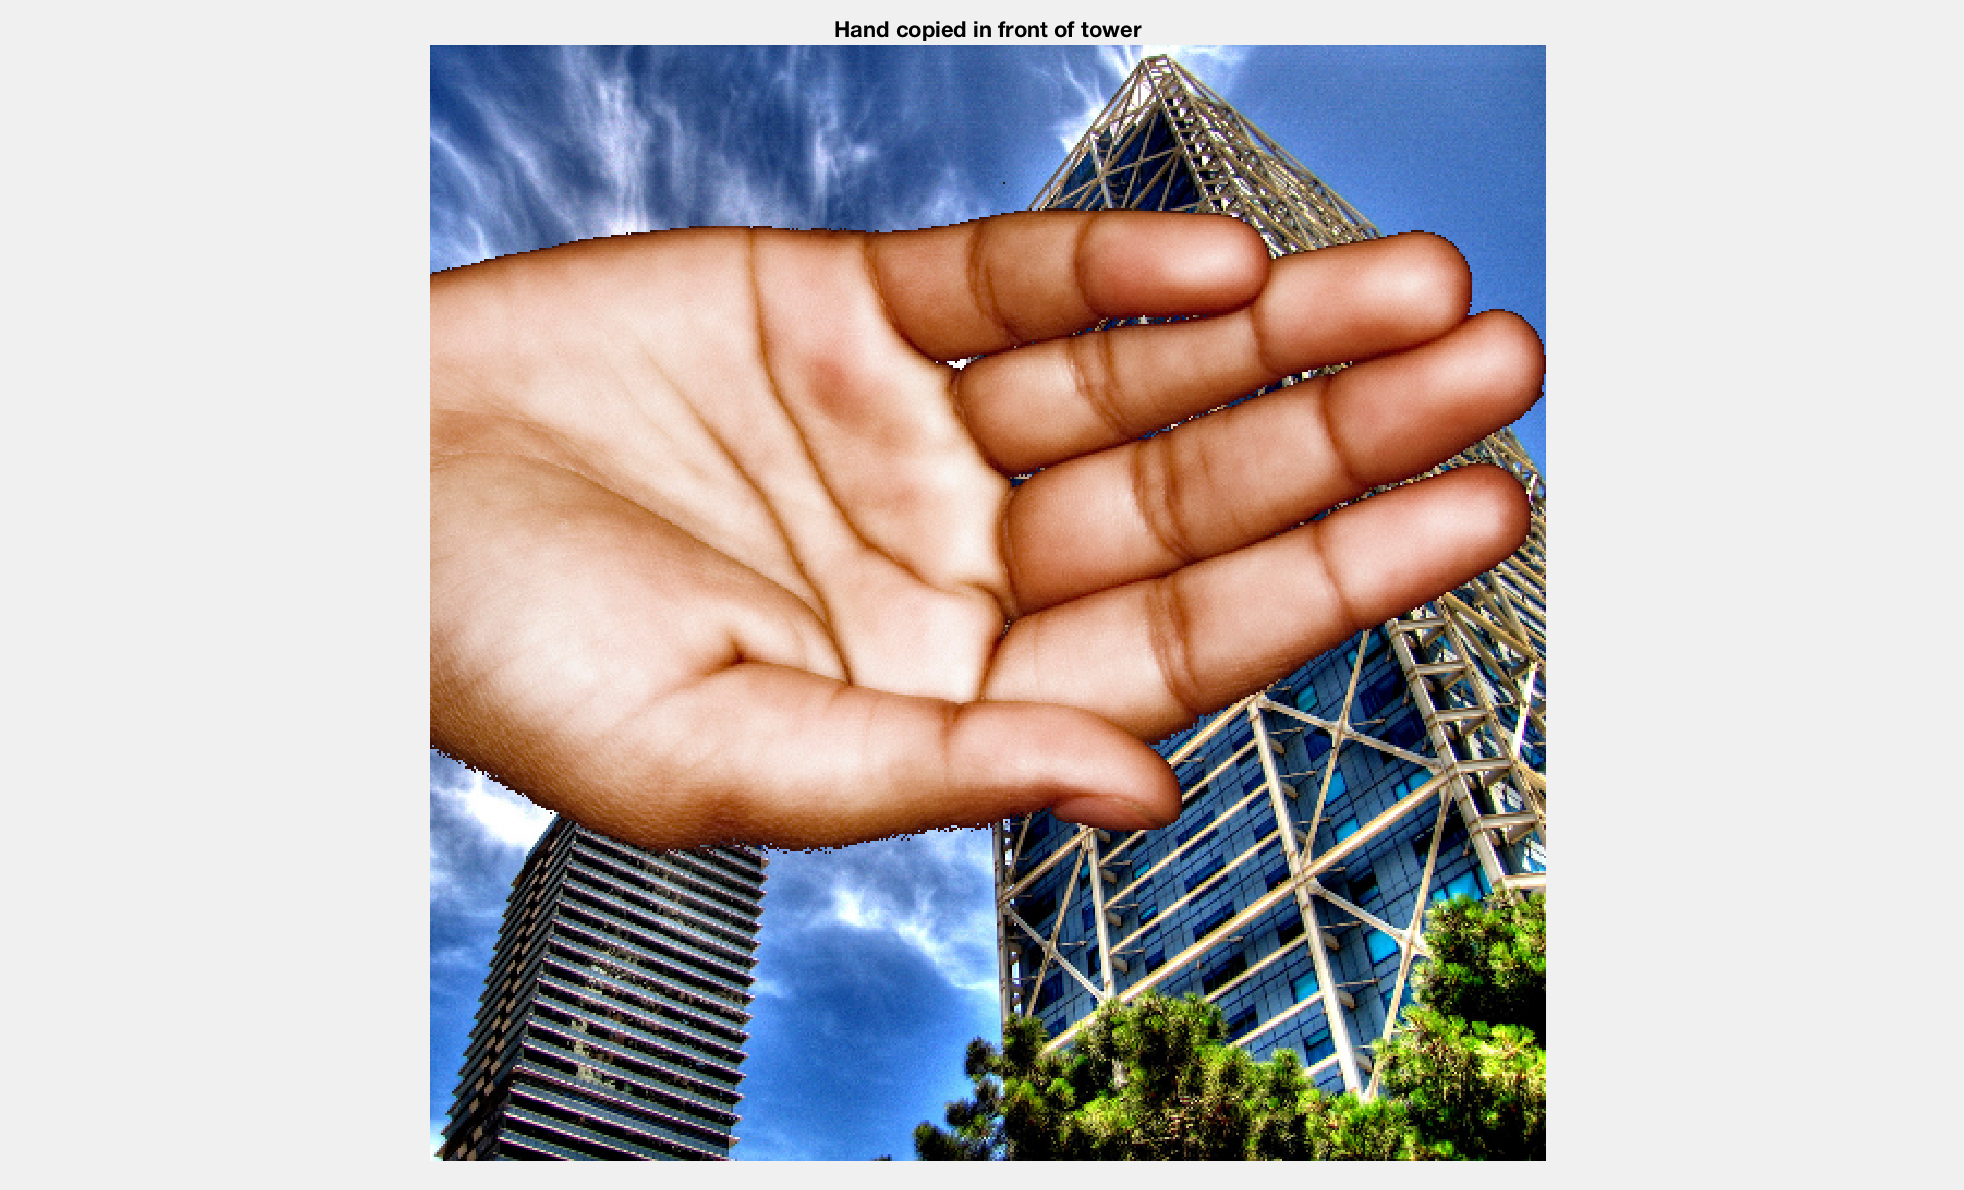
\includegraphics[width=\textwidth]{./img/task22.png}
  \caption{Hand copied in front of tower}
  \label{fig:task22}
\end{figure}